\section{Integration checks and remaining validity boundaries}
\label{sec:theory-audit}
The working model now adopts the geometric mixture in
Eq.~\eqref{eq:relative-forward-directed} and the training-global relative
threshold in Eq.~\eqref{eq:relative-consistency-threshold}.
All construction and search definitions in Sections 2--3 refer to this
same model, including the training-internal predictive guard in
Section~\ref{sec:cost-reduction}. Historical information-only and absolute-threshold settings
are retained only as clearly labeled diagnostics.

\subsection{Recovery of the repeated-XOR construction}
Take two binary categorical attributes $a,b$, repeat every value pair
twice, and assign $(0.9,0.1)$ when $a=b$ and $(0.1,0.9)$ otherwise.
Every individual attribute value has mean label profile $(0.5,0.5)$,
equal to the global mean. Hence every marginal information weight and
categorical label-profile discrepancy is zero. The information-only
predecessor therefore has zero distance even on the joint subset.
Nonpositive-gain search alone cannot recover this erased geometry.

The adopted geometric term preserves distinct joint attribute vectors.
With $\zeta=0.1$, $\kappa=0.1$, $s_{\min}=2$, $\alpha=1$ and zero
improvement tolerances, the reference construction gives
\[
\Gamma(\{a\})=\Gamma(\{b\})=0,\qquad\Gamma(\{a,b\})=1.
\]
Both searches reach the feasible pair in this example; the heuristic
first takes a zero-gain bridge. This verifies a particular interaction
recovery, not a universal interaction-detection guarantee.
\begin{figure}[htbp]
\centering
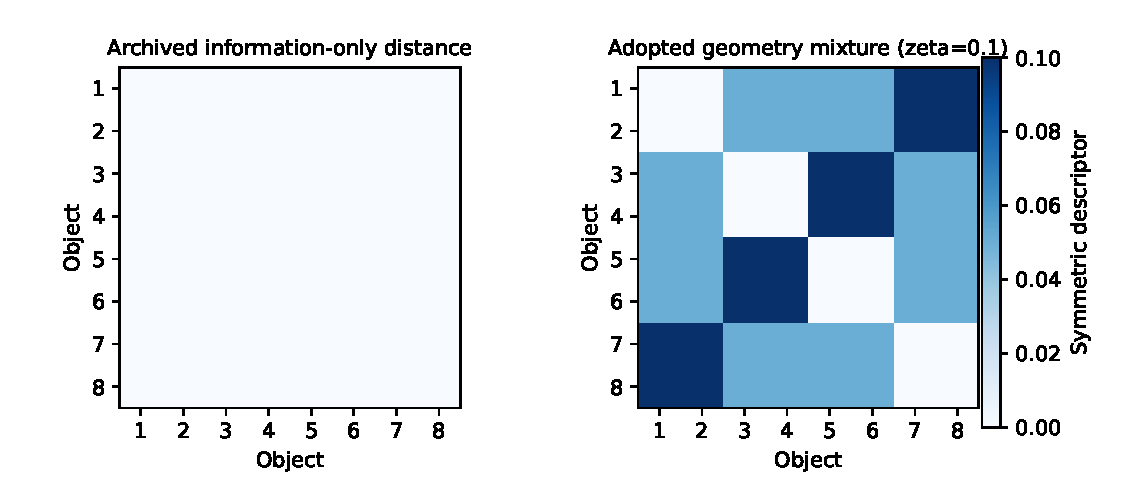
\includegraphics[width=\linewidth]{theory_audit_xor.pdf}
\caption{Archived information-only geometry and adopted mixed geometry
on the same eight-object construction. The geometric component preserves
joint attribute distinctions that marginal label profiles erase.}
\end{figure}

\subsection{Relative consistency avoids premature root stopping}
For categorical values $(A,A,B,B)$, assign distributions
$(0.5+0.4t,0.5-0.4t)$ at A and $(0.5-0.4t,0.5+0.4t)$ at B,
where $0<t\le1$. The global variation is $V_0=0.32t^2$.
An absolute threshold $\delta\ge V_0$ with inactive radius gate makes
an uninformative root eligible and stops construction prematurely.
The adopted $\delta=\kappa V_0$ with $\kappa<1$ prevents this mechanism
for every $V_0>0$. Holding the adopted distance fixed, the checks give:
\begin{center}
\begin{tabular}{cccc}
\hline
$t$ & $V_0$ & Archived fixed $\delta=0.01$ & Adopted $\delta=0.1V_0$\\
\hline
1 & 0.32 & $\Gamma=1$ & $\Gamma=1$\\
0.25 & 0.02 & $\Gamma=1$ & $\Gamma=1$\\
0.1 & 0.0032 & $\Gamma=0$ & $\Gamma=1$\\
\hline
\end{tabular}
\end{center}
This does not establish invariance of the full method under label
rescaling: KL weights and geometry can change. Very small $V_0$ can
still amplify sampling noise in normalized dependency.

\subsection{Properties rechecked after integration}
The supplied cross-checks verify bounds, zero diagonal, attribute
monotonicity, genuine directional differences, inactive-label handling,
constant-attribute contributions, numerical and categorical signal
examples, and completed search agreement with exhaustive enumeration.
The numerical counterexample in Section~\ref{subsec:ldl-directed} is
verified at $\zeta=0.001,0.1,0.5,0.99$; its algebra proves triangle
failure for every $0<\zeta<1$ in that construction.
The reconstructed negative gain in Section~\ref{subsec:granulation-rule}
is recomputed under the adopted parameters, not copied from the predecessor.

The proofs of variance decomposition, finite construction, fixed-subset
construction monotonicity, heuristic single-deletion irreducibility and
completed exact-search optimality remain valid. None of them implies
adaptive attribute-dependency monotonicity or generalization.
The max-of-directions splitting descriptor is symmetric; an ablation
must assess what source-dependent information weights contribute rather
than claiming an asymmetric traversal algorithm.

\subsection{Unified diagnostic parameters}
These settings define a reproducible starting configuration, not
empirically optimal hyperparameters.
\begin{center}
\begin{tabular}{p{0.22\linewidth}p{0.65\linewidth}}
\hline
Parameter & Working convention and interpretation\\
\hline
$\tau_a>0$ & Numerical bandwidth: median positive pairwise difference of
training-normalized values. Constant attributes contribute zero.\\
$\beta=1$ & Local-profile shrinkage, fixed across subsets.\\
$\zeta=0.1$ & Adopted geometric mixture; $\zeta=0$ is only an ablation.\\
$s_{\min}=2$ & Diagnostic support lower bound; study larger values for
larger training samples.\\
$\kappa=0.1$ & Relative consistency: $\delta=\kappa V_0$, fixed per fold.\\
$\alpha=1$ & Radius eligibility gate inactive; radius remains a descriptor
and a split-improvement signal.\\
$\varepsilon_V=\varepsilon_r=0$ & Exact split-improvement rule; explicitly
report any positive numerical tolerance.\\
$\epsilon=0$ & Exact dependency preservation for mechanism checks;
distinct from split tolerances.\\
$\lambda=-1$ & Positive gain per test cost; affects the heuristic path.\\
\hline
\end{tabular}
\end{center}
All statistics are fitted on training objects. When tuning, refit them
within each inner training fold. Validation labels evaluate held-out losses
but do not enter their associated training geometry or ball centers.
The reference implementation also supports numerical and categorical
attributes using the same local-profile estimator.

An active radius gate has cardinality dependence because $r_P\le|P|/m$.
Under the working $\alpha=1$ and $\varepsilon_r=0$, padding with constant
attributes only rescales every distance by a common positive factor:
seed and medoid ordering, radius-improvement signs and label-based
eligibility remain unchanged, hence so does the partition. This is also
checked numerically. The fixed $m$ denominator is retained; replacing it
by $|P|$ would invalidate the established monotonicity proof.

\subsection{Remaining empirical questions}
The marginal information term can be noisy, self-influenced or redundant;
rare active label masses affect its normalizer. Geometric contributions
can include irrelevant attributes. Hard eligibility thresholds are
sensitive near their boundaries, and the single farthest-seed candidate
can fail support when another split would work. These limitations have
not been removed by the two adopted revisions.

The dense reference code caches per-attribute matrices in $O(mn^2)$
memory and computes Gaussian weighted label means in up to
$O(mn^2q)$ time. It validates definitions, not scalability. Numerical
tolerances and memory optimizations require explicit specification before
large-dataset experiments.

If the reference dependency or preservation threshold is zero, report
the weak reference separately. Under the working joint objective the
empty set must additionally pass the inner predictive guard. Relative excess-cost metrics dividing by an
optimum of zero are not applicable; do not interpret an empty optimal
subset as predictive success. A timed-out exact search supplies only a
feasible incumbent. Future evidence must combine held-out LDL losses,
reduction cost, coverage, leaf structure and runtime on real LDL datasets.
The checked constructions are theoretical diagnostics, not substitutes
for those experiments.
